\chapter{Аналитический раздел}

\section{Формализация задачи}

Для исследования получаемого в зеркале изображения будет смоделирована сцена, состоящая из следующих объектов:
\begin{itemize}
	\item композиция геометрических объектов, выбираемых пользователем (для
	выбора доступны сфера, куб, правильная усеченная четырехгранная пирамида, правильная трехгранная призма);
	\item платформа, на которой стоят геометрические объекты;
	\item плоское зеркало, свойства которого являются целью изучения;
	\item точечный источник освещения, задаваемый координатами положения и интенсивностью.
\end{itemize}

Геометрические объекты будут задаваться минимально достаточным набором информации:
\begin{itemize}
	\item сфера -- координаты центра и радиус;
	\item куб -- координаты левой нижней ближайшей вершины, длина ребра и угол поворота вокруг оси Oy;
	\item усеченная пирамида -- координаты левой нижней ближайшей вершины, длина основания, высота неусеченной версии пирамиды и высота усеченной (если исходная высота оказывается меньше усеченной, строится обычная четырехгранная пирамида высотой, равной наименьшему из двух значений);
	\item призма -- координаты левой нижней ближайшей вершины, длина основания, высота призмы.
\end{itemize}
Наиболее удобным представлением вышеперечисленных объектов, за исключением сферы, будет полигональная сетка в виде списка граней. Также для каждой фигуры задается цвет RGB-тройкой и характеристики материала (т.е. свойствами взаимодействия со светом): коэффициент отражения, зеркальность и шероховатость поверхности.

Также необходимо реализовать камеру, задаваемую координатами местоположения и вектором, определяющим направление взгляда.

Для того, чтобы поставленная задача реализовывалась быстро, независимо от меняющихся объектов, источников освещения и покрытия плоского зеркала, необходимо выбрать алгоритмы, которые будут максимально эффективны в данном случае.

\section{Алгоритмы построения изображения}

Чтобы правильно построить изображение, необходимо воспользоваться алгоритмом, который будет корректно и быстро удалять невидимые линии и поверхности. Некоторые алгоритмы работают в объектном пространстве, в таком случае мы имеем дело с мировой системой координат. Другие же оперируют в пространстве изображения -- экранная система координат \cite{alg_3d_graph}. Рассмотрим часто используемые алгоритмы и выберем оптимальный.

\subsection{Алгоритм Робертса}

Данный алгоритм работает в объектном пространстве и только с выпуклыми телами. В случае невыпуклых тел необходимо сначала провести разбиение его на выпуклые.

Для каждого объекта формируется матрица тела — для каждой грани вычисляются коэффициенты уравнения плоскости, проходящей через нее, после необходимо проверить матрицу на корректность \cite{rodz}.

Первоочередно в алгоритме удаляются грани и ребра, экранируемые самим телом, в дальнейшем — другими телами. При этом возможны несколько случаев:
\begin{itemize}
	\item ребро полностью невидимо;
	\item ребро полностью видимо;
	\item ребро экранируется частично, в таком случае ребро разбивается на несколько частей.
\end{itemize}

Преимуществом данного алгоритма является использование математических методов, которые просты и обладают высокой точностью.

Главным недостатком является рост сложности алгоритма. Ее зависимость представляет собой квадрат числа всех объектов сцены. Также если рассматривать уже оптимизированные варианты алгоритмов, их реализация оказывается достаточно трудоемкой \cite{alg_comp_graph}.

\subsection{Алгоритм Варнока}

Данный алгоритм работает в пространстве изображения, разбивая картинную плоскость на части (области), для каждой из которых исходная задача может быть решена относительно просто.

Для каждой части определяются связанные с ней многоугольники, и полностью видимые из их числа отображаются на экране. В ином случае область разбивается на подобласти до тех пор, пока не достигнется простая видимость или же область не станет размером в 1 пиксель. Предполагается, что чем меньше область, тем меньше многоугольников ее перекрывают. Однако если полученная область в 1 пиксель все еще перекрыта несколькими многоугольниками, определяется глубина каждого из них и визуализируется находящийся ближе к наблюдателю.

Объективным преимуществом является простота понимания алгоритма, однако анализ картинной плоскости с последующим ее разбиением и отображением может занять большое количество времени \cite{alg_comp_graph}.

\subsection{Алгоритм, использующий Z-буфер}

Данный алгоритм работает в пространстве изображения. В ходе его работы значение z-координаты (глубины) каждого нового пикселя, заносимого в буфер кадра, сравнивается с z-координатой пикселя уже занесенного в Z-буфер. Если сравнение показывает на то, что новый пиксель располагается ближе к наблюдателю, то Z-буфер обновляется, а также корректируется значение интенсивности в буфере кадра \cite{rodz}.

Алгоритм является одним из простейших в реализации. Его сложность линейно зависит от сложности сцены. Также алгоритм Z-буфера позволяет рассматривать объекты сцены в произвольном порядке, не затрачивая время на их сортировку.

Несмотря на подобную простоту и удобство алгоритма, он является затратным по памяти, так как нам приходится хранить буфер кадра и Z-буфер для попиксельного хранения изображений.

\subsection{Алгоритм прямой трассировки лучей}

Данный алгоритм работает в пространстве изображения. Для каждого пикселя картинной плоскости определяется ближайшая к нему грань, это производится выпусканием луча и нахождением всех его пересечений с гранями. Так как объекты могут отражать, поглощать или пропускать лучи света сквозь себя, необходимо учитывать все образующиеся лучи. 

Для каждого первичного луча строится дерево трассировки, ветви которого составляют вторичные лучи. Ветвление заканчивается, когда луч вышел за пределы сцены, встречается с непрозрачным телом, попадает в источник света, когда интенсивность падает ниже порога чувствительности или когда расщепление первичного луча становится слишком велико.

Из преимуществ можно отметить то, что достигается высокая реалистичность получаемого изображения. Помимо этого каждый луч можно рассматривать независимо от остальных, что предоставляет возможность для распараллеливания выполнения построений.

Однако низкая производительность является серьезным недостатком. Для получения изображения приходится выпускать множество лучей, проходящих через сцену и отраженных от объектов \cite{alg_comp_graph}.

\subsection{Алгоритм обратной трассировки лучей}

Метод обратной трассировки лучей исправляет главный недостаток прямой трассировки -- большое количество испускаемых лучей. 

Строится путь светового луча от приемника к объекту и источнику. Данный метод аккумулирует все лучи, в действительности приходящие в приемник из определенного направления независимо от их начала. Количество лучей ограничено числом точек на поверхностях объектов сцены, видимых из точки наблюдения, поэтому вычислительные затраты значительно уменьшаются по сравнению с методом прямой трассировки.\newline

\textit{Вывод:} Для реализации выбран алгоритм обратной трассировки, так как он позволяет учесть все особенности поверхностей фигур. Также данный метод является одним из этапов построения отражения в плоском зеркале, который будет рассмотрен далее.

%\section{Алгоритмы закраски}

%Закраска изображения позволяет отобразить глубину за счет различного уровня освещения в разных точках. Выбор цвета может зависеть от расстояния до источника света, угла падения лучей, положения наблюдателя.

%\subsection{Метод Гуро}

%Данный вид закраски использует интерполированные значения интенсивности, благодаря чему достигается сглаженность изображения. В основе метода лежит закрашивание плавно меняющимися оттенками, вычисление которых получается билинейной интерполяцией интенсивностей примыкающих граней.

%При реализации необходимо вычислить нормали к каждой имеющейся грани, после чего определить усредненные нормали к вершинам (усреднить значения нормалей примыкающих граней). Далее вычисляются интенсивности в вершинах. После чего уже закрашивается грань полученным на основе интерполяции вершин цветом.

%Главным недостатком метода является появление полос Маха \cite{alg_3d_graph}. Это явление заключается в изменении интенсивности при фактически постоянной освещенности, а также то, что при линейной интерполяции значение интенсивности на некоторых участках может получится равной, и поверхность на данных участка будет выглядеть плоской.

%\subsection{Метод Фонга}

%Данный метод строится по тому же принципу, что и метод Гуро. Главное отличие заключается в том, что используется билинейная аппроксимация не для интенсивностей, а для векторов нормалей к граням.

%При реализации сначала вычисляются нормали к каждой грани, затем определяются усредненные нормали к вершинам, а дальше вычисляются интерполированные векторы нормали в каждой точке грани, и уже на ее основе определяется интенсивность в каждой точке.

%Недостатками являются большой объем вычислений и больший эффект полос Маха на сферах, хотя на других телах он проявляется меньше. Помимо этого, оба метода приводят к ошибкам при закраске невыпуклых многоугольников, потому что нарушается равномерность закраски \cite{alg_3d_graph}. \newline

%\textit{Вывод:} При реализации поставленной задачи будет использован алгоритм закраски по Фонгу, так как он позволит достичь большей реалистичности полученного изображения и учесть все особенности текстуры поверхностей (их зеркальные и диффузные составляющие). 

\section{Модели освещения}

Для моделирования освещения трехмерных объектов используются различные модели освещения. Рассмотрим основные из них.

\subsection{Модель Ламберта}

Модель Ламберта --- одна из простых моделей освещения, которая представляет собой комбинацию фоновой и диффузной составляющих. Поверхность при такой модели будет выглядеть одинаково ярко со всех направлений наблюдений. Интенсивность имеет вид:
\begin{equation}
	I = I_{a} + I_{d},
\end{equation}
где $I_{a}$ -- фоновая составляющая (ambient), $I_{d}$ -- рассеянная составляющая (diffuse).

\begin{figure}[H]
	\begin{center}
		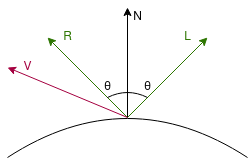
\includegraphics[scale=0.8]{assets/i_ray.png}
	\end{center}
	\caption{Схема рассматриваемых при падении лучей}
	\label{i_ray}
\end{figure}

Фоновое освещение --- постоянная в каждой точке величина надбавки к освещению. Вычисляется как:
\begin{equation}
	I_{a} = k_{a} \cdot i_{a},
\end{equation}
где $k_{a}$ -- свойство материала воспринимать фоновое освещение, $i_{a}$ -- мощность фонового освещения. Чаще всего задается некое глобальное фоновое освещение всей сцены.
Схожим образом рассчитывается и диффузная составляющая освещения:
\begin{equation}\label{id}
	I_{d} = k_{d} \cdot i_{d} \cdot cos(\vec{L}, \vec{N}),
\end{equation}
где $k_{d}$ -- свойство материала воспринимать рассеянное освещение, $i_{d}$ -- мощность рассеянного освещения, $\vec{L}$ -- луч, обратный падающему, $\vec{N}$ -- нормаль к точке поверхности (рисунок \ref{i_ray}). 

Для удобства рассмотренные векторы можно взять как единичные, тогда косинус угла между ними совпадает со скалярным произведением и формула (\ref{id}) примет вид:
\begin{equation}
	I_{d} = k_{d} \cdot i_{d} \cdot (\vec{L}, \vec{N}).
\end{equation}

\subsection{Модель Фонга}

Модель Фонга --- классическая модель освещения. Представляет собой комбинацию  фоновой, диффузной составляющей (модели Ламберта) и зеркальной составляющей, работает таким образом, что кроме равномерного освещения на материале может еще появляться блик.Его местонахождение определяется из закона равенства углов падения и отражения.

В данной модели интенсивность имеет вид:
\begin{equation}\label{intensity}
	I = I_{a} + I_{d} + I_{s},
\end{equation}
где $I_{a}$ -- фоновая составляющая (ambient), $I_{d}$ -- рассеянная составляющая (diffuse), $I_{s}$ -- зеркальная составляющая (specular).

Формула для зеркальной составляющей имеет вид:
\begin{equation}\label{is}
	I_{s} = k_{s} \cdot i_{s} \cdot cos^\alpha(\vec{R}, \vec{V}),
\end{equation}
где $k_{s}$ -- коэффициент зеркального отражения, $i_{s}$ -- мощность зеркального освещения, $\vec{R}$ -- направление отраженного луча, $\vec{V}$ -- направление на наблюдателя (рисунок \ref{i_ray}), $\alpha$ -- коэффициент блеска материала поверхности.

В случае единичных векторов формула (\ref{is}) принимает вид:
\begin{equation}
	I_s = k_s \cdot i_s \cdot (\vec{R}, \vec{V}).
\end{equation}\newline

\textit{Вывод:} При решении будет использоваться модель Фонга, так как она учитывает все интересующие в ходе данной работы составляющие освещения.

%\subsection{Локальная модель}

%Данная модель не рассматривает взаимодействие объектов между собой, только расчет освещенности самих объектов. В рамках локальной модели освещения играет значение лишь свет от явных точечных источников света, взаимодействие ограничивается однократным отражением света от непрозрачной поверхности. Изображение формируется в результате падающего на поверхность объектов света, интенсивность и цвет которого и необходимо рассчитать.

%\subsection{Глобальная модель}

%Данная модель рассматривает трехмерную сцену как одну систему и описывает освещение с учетом взаимодействия объектов между собой. В рамках глобальной модели освещения учитывается множество явлений, таких как многократное отражение, преломление света, рассеянное освещение и прочее. Является более точной и реалистичной.\newline

%\textit{Вывод:} При реализации поставленной задачи будет использоваться локальная модель освещения, так как учет взаимодействия объектов сцены между собой не является целью изучения. Для изучения отражающей способности покрытия зеркала этой модели будет вполне достаточно. Также это сократит время выполнения отображения.

\section{Визуализация размытых отражений}

В данной работе изучается диффузная составляющая покрытия зеркала, а значит показатель ее шероховатости будет изменять отраженные от объектов лучи, и изображение будет принимать другой вид.

При построении размытого отражения, в отличие от отражения идеального зеркала, для отраженного луча выбирается произвольное направление в некотором конусе, ось которого совпадает с вектором идеально отраженного луча, а радиус зависит от диффузной составляющей покрытия. Итоговое значение интенсивности может быть найдено, как среднее от значений, полученных для каждого выпущенного луча.

Чтобы избежать трудоемких операций с синусами и косинусами, можно аппроксимировать конус четырехугольной пирамидой, высотой которого является вектор идеально отраженного луча. Основание будет перпендикулярно отраженному лучу, а длина его стороны будет зависеть от шероховатости поверхности -- чем больше диффузная составляющая, тем больше сторона, а значит и отражение менее четкое.\newline

%Поверхность зеркала рассматривается как набор случайных микрограней, предполагаемый размер которых намного меньше пикселя, поэтому не заметна гранулярность. В целом этот метод дает хорошее приближение, достаточное для фотореалистичного внешнего вида \cite{fuzzy_refflection}.

%Визуализация размытых отражений базируется на основе двухпроходного рендеринга. Первым этапом является обычная обратная трассировка \cite{rodz}, предполагающая зеркальное (полное) отражение.

%После данного этапа для каждого пикселя мы будем знать: физическую яркость $L_{0}$ зеркального отражения; координаты точки пересечения на зеркальной поверхности; координаты точки попадания идеального отражения луча на поверхность сцены. Второй этап заключается в «фильтрации» изображения, что означает, что для тех пикселей, точка пересечения которых принадлежит зеркальной поверхности вычисляется следующая функция:
%\begin{equation}
%	L(x, y) = \frac{\sum\limits_{y', x'} L_{0}(x', y') f(x, x', y, y')}{\sum\limits_{y', x'} f(x, x', y, y')},
%\end{equation}
%где $L_{0}(x, y)$ – яркость изображения в пикселе $(x, y)$; $L(x, y)$ – результирующая яркость, которая представляет нечеткое отражение; $f(x, x’, y, y’)$ - весовые коэффициенты, зависящие от свойств материала и угла $\vartheta$ (на рис. 1 \textbf{РИСУНОК ДОБАВИТЬ}).

%Весовые коэффициенты легко находятся по формуле:
%\begin{equation}
%	f = pow(cos\vartheta, p),
%\end{equation}
%где $p$ – коэффициент Фонга (зеркальности), а $\vartheta(x, x’, y, y’)$ - угол между направлениями от точки пересечения до конца данного луча и луча отраженного от данной точки до конца от соседнего пикселя $(x’, y’)$. При этом $cos\vartheta$ находится следующим способом:
%\begin{equation}
%	cos\vartheta(x, x', y, y') = \frac{(b(x', y') - a(x, y), b(x, y) - a(x, y))}{|b(x', y') - a(x, y)| \cdot |b(x', y') - a(x, y)|},
%\end{equation}

%Предполагается, что поверхность близка к зеркальной, (3) поэтому отраженная энергия располагается под углом $\vartheta \leq \theta \leq 10^{\circ}$. В таком случае влиянием дальних пикселей можно пренебречь. Отсюда формула (1) может вычисляться по соседним с $(x, y)$ пикселям. Лучи, отраженные от них, и от камеры до центрального пикселя $(x, y)$ находятся под углом, меньшим чем:
%\begin{equation}
%	\alpha = \frac{\theta}{1 + s / r},
%\end{equation}
%где $s$ – расстояние от камеры до центрального пикселя $(x, y)$, $r$ – расстояние от последнего до конца отраженного луча. По угловому размеру нетрудно оценить радиус в пикселях:
%\begin{equation}
%	\rho = \alpha \cdot (\text{размер изображения}) / (\text{угол обзора}).
%\end{equation}

%В равной степени мы можем использовать как прямоугольную, так и круглуюобласть, с полученным радиусом.

\section{Вывод из раздела}

В данном разделе были рассмотрены алгоритмы построения реалистичного изображения. При реализации поставленной задачи будут использоваться алгоритмы обратной трассировки лучей, модель освещения Фонга. Обратная трассировка также ляжет в основу алгоритма построения размытых отражений.